\documentclass{mcmthesis}
\mcmsetup{CTeX = true,   % 使用 CTeX 套装时,设置为 true
        tcn = XJ162, problem = A,
        sheet = true, titleinsheet = true, keywordsinsheet = true,
        titlepage = false, abstract = false}
\geometry{left=1in,right=0.75in,top=1in,bottom=1in}
\numberwithin{figure}{section}
\numberwithin{table}{section}
\numberwithin{equation}{section}
\usepackage{newtxtext}
\usepackage{lipsum}
\usepackage{palatino}
\usepackage{hyperref}
\usepackage{booktabs}
\usepackage{subfigure}
\usepackage{graphicx}
\usepackage{pythonhighlight}
\usepackage{indentfirst}%首段自动缩进
\usepackage{colortbl}
\usepackage{apacite}
\usepackage{natbib}


\setlength{\parindent}{2em}
\title{test}
\setlength{\headheight}{15pt}

\definecolor{darkOrange}{rgb}{0.929,0.49,0.192}
\definecolor{Orange}{rgb}{0.973,0.796,0.678}
\definecolor{lightOrange}{rgb}{0.988,0.894,0.839}

\begin{document}

\begin{abstract}



\begin{keywords}
123456
\end{keywords}
\end{abstract}
\maketitle

\tableofcontents
  \thispagestyle{empty}
  \newpage
  \setcounter{page}{1}
%%
%%Generate the Memorandum, if it's needed.
%\memoto{\LaTeX{}studio}
%\memofrom{Liam Huang}
%\memosubject{Happy \TeX{}ing!}
%\memodate{\today}
%%\logo{\LARGE I'm pretending to be a LOGO!}
%\begin{memo}[Memorandum]
%  \lipsum[1-3]
%\end{memo}

\section{Introduction}

\subsection{Problem Restatement}

Finless porpoise is the only freshwater mammal in the Yangtze River at present, 
which is distributed in the middle and lower reaches of the Yangtze 
River, Dongting Lake and Poyang Lake, and its population has 
decreased dramatically in the past 20 years. According to the statistics, 
the number of finless porpoises in the Yangtze River was more than 2,700 in 1991. 
However, in the year of 2006, there were fewer than 1,800 finless porpoises surviving in the area. 
In 2011, there were probably just over 1,000 of them, and in 2018 there were about 1,012. 
\par
In fact, since the 1980s, the ecologists along with the government
had explored and developed three conservation strategies: 
in situ conservation, ex situ conservation and artificial breeding.
Among them, ex situ protection, that is, selecting some waters with 
similar ecological environment to the Yangtze River to establish 
ex situ protection, is the most direct and effective measure
to protect the Yangtze finless porpoise. 
\par
China has set up five ex-situ protected sites until now, in which 
more than 150 Yangtze finless porpoises are conserved. On September 18, 2021, CCTV reported that 
the population of the Yangtze finless porpoise is growing steadily. 
The population decline of the Yangtze finless porpoise has been 
curbed, but its critically endangered status remains unchanged.
\par
Based on what has been discussed above, please address the following problems:
\begin{enumerate}
  \item [1] Establish a mathematical model to predict the population number of finless porpoises in five ex situ protected areas after 20 years, 
  and explain how the sex ratio of 150 finless porpoises in ex situ protected areas affects the population development of finless porpoises.
  \item [2] Will the Yangtze finless porpoise become functionally extinct without ex situ conservation strategies?
  \item [3] Based on your analysis, please submit no more than 2 pages of recommendations for the protection of finless porpoises to the relevant authorities.
\end{enumerate}

\subsection{Overview of Our Work}




\section{Assumptions and Justifications}



\section{Notations}

\renewcommand\arraystretch{1.5}

\begin{table}[htpb!]
  \centering
  \caption{Notation Descriptions} \label{Varibles}
  \begin{tabular}{m{2.5cm}<{\centering}|m{12.5cm}<{\centering}}
  \toprule[1.5pt]
  \textbf{Symbol} & \textbf{Definition} \\ \hline
  $\mathbf{A}$ & A set of artists given in dataset \\
  $\mathbf{G}$ & A set of genres provided in dataset \\
  $f_i$ & The total number of followers of artist $i$, $i\in \mathbf{A}$ \\
  $g_{ij}$ & Genre tag between artist $i$ and his or her follower $j$, $i,j \in \mathbf{A}$ \\
  $DAS_{i}$ & Artist $i$'s decade of active start, accurate to 10 years \\
  $r_{ij}$ & Respective Influence of influencer $i$ over follower $j$, $i,j \in \mathbf{A}$ \\
  $w_{i}$ & Artist $i$'s weight of normalized indexes \\ 
  $TI_{i} $ & Artist $i$'s Total Influence \\
  $wf_j$ & The parameter of follower $j$' influence, $j\in \mathbf{A}$ \\
  $wt_{i}$ & The weight of artist $i$'s Total Influence, $i,j\in \mathbf{A}$\\
  $cg_{ik}$ & Artist $i$'s Contemporary Influence in certain genre, $i\in \mathbf{A}, k \in \mathbf{G}$ \\
  $c_{i}$ & Artist $i$'s Contemporary Influence, $i\in \mathbf{A}$ \\
  $S_{ij} $ & Similarity between artists $i$ and $j$ \\
  \bottomrule[1.5pt]
  \end{tabular}
  \end{table}




\section{Model I:}

Considering tremendous cost on massive finless porpoise population 
census, merely six years of data was collected during the three 
decades since 1992. \citep{Liuzhigang}
Thus, we've applied \textbf{Lagrange interpolation} to obtain other years' data.

\subsection{Lagrange Interpolation}
Given $ n $ distinct real values $ x_1, x_2, \cdots , x_n $and $ n $
real values $ y_1, y_2,\cdots, y_n $ (not necessarily distinct), there
is a unique polynomial $ P $ with real coefficients satisfying 
$ P(x_i)= y_i $ for $ i \in \{1,2,\cdots,n\} $, such that deg($ P $ )<n.
\par
The polynomial $ P(x) $ is defined as follows:   
$$
  P(x) = \sum \limits _{k = 1}^ny_kp_k(x),\quad
  p_k(x) = \frac{(x-x_1)\cdots (x-x_{k-1})(x-x_{k+1})\cdots (x-x_n)}{
    (x_k-x_1)\cdots (x_k-x_{k-1})(x_k-x_{k+1})\cdots (x_k-x_n)
  }
$$
According to Lagrange interpolation, the number of finless porpoise population 
during past three decades are listed below.
\begin{table}[htpb!]
  \centering
  \caption{Estimated size of population on year basis from 1992 to 2022} \label{Lagrange table}
  \begin{tabular}{m{2cm}<{\centering}|m{2cm}<{\centering}|m{2cm}<{\centering}|m{2cm}<{\centering}|m{2cm}<{\centering}|m{2cm}<{\centering}}
  \rowcolor{darkOrange}  \textbf{Year}&\textbf{Number}&\textbf{Year}&\textbf{Number}&\textbf{Year}&\textbf{Number}\\ \hline
  \rowcolor{Orange}  1992 & 5       & 2002 & 20      & 2012 & 45.7364 \\
  \rowcolor{lightOrange}  1993 & 10.4864 & 2003 & 21.2919 & 2013 & 49.2555 \\
  \rowcolor{Orange}  1994 & 13.9987 & 2004 & 22.9647 & 2014 & 52.9737 \\
  \rowcolor{lightOrange}  1995 & 16.0839 & 2005 & 25      & 2015 & 57      \\
  \rowcolor{Orange}  1996 & 17.2014 & 2006 & 27.3612 & 2016 & 61.4941 \\
  \rowcolor{lightOrange}  1997 & 17.7296 & 2007 & 30      & 2017 & 66.6734 \\
  \rowcolor{Orange}  1998 & 17.9732 & 2008 & 32.8636 & 2018 & 72.82   \\
  \rowcolor{lightOrange}  1999 & 18.1701 & 2009 & 35.9015 & 2019 & 80.2876 \\
  \rowcolor{Orange}  2000 & 18.4981 & 2010 & 39.0724 & 2020 & 89.5084 \\
  \rowcolor{lightOrange}  2001 & 19.0819 & 2011 & 42.3514 & 2021 & 101     \\
  \end{tabular}
\end{table}


\begin{figure}[htbp!]
  \centering

  \subfigure[caption1]{
  \centering
  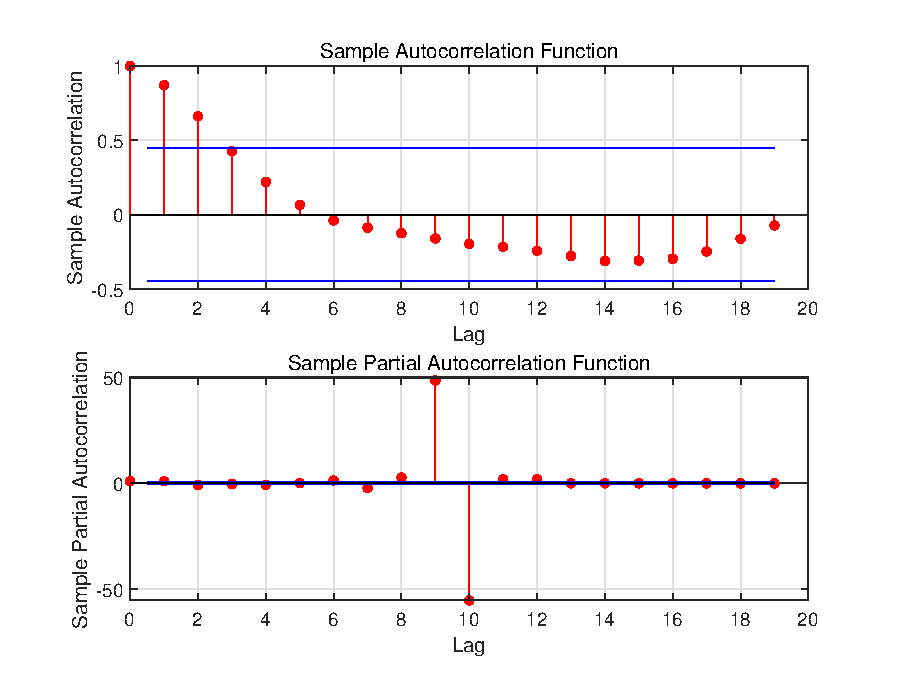
\includegraphics[width = 6cm]{codes/1.eps}
\quad

  }
  \subfigure[caption2]{
  \centering
  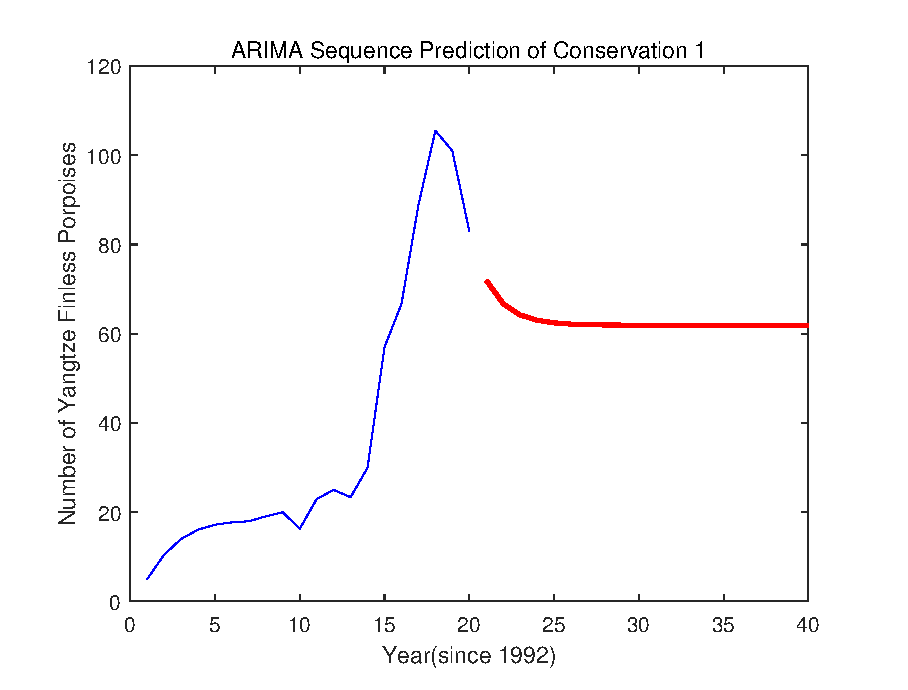
\includegraphics[width = 6cm]{codes/2.eps}
  }
\quad

\subfigure[caption3]{
  \centering
  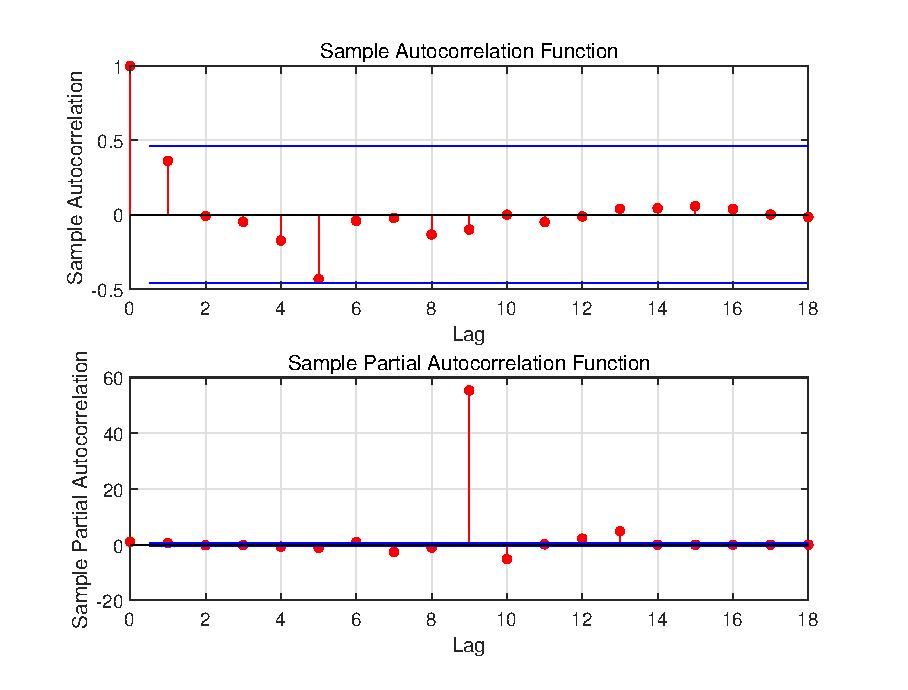
\includegraphics[width = 6cm]{codes/3.eps}
}

\end{figure}

\begin{figure}[htbp]
  \centering
  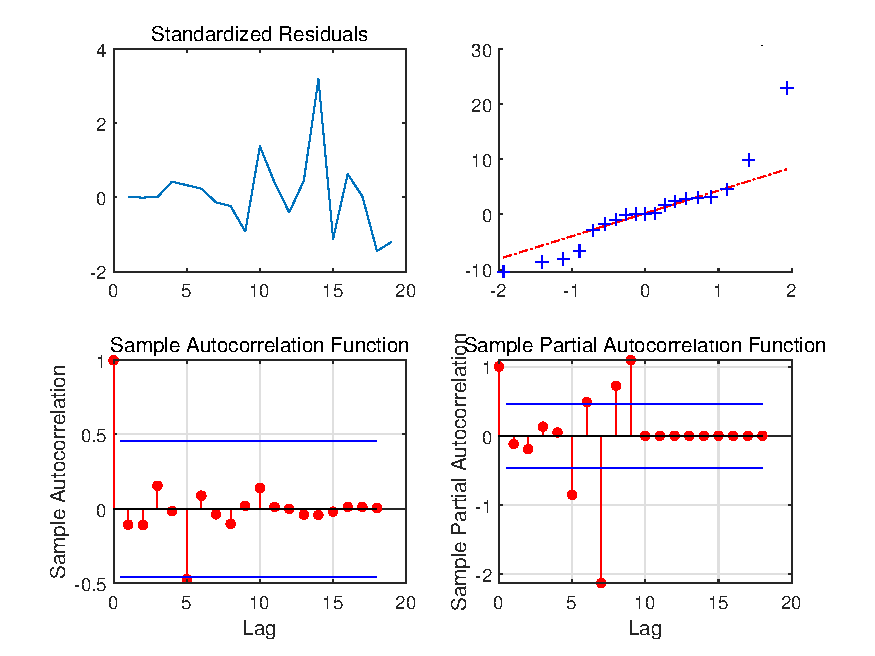
\includegraphics{codes/4.pdf}
  \caption{caption4}

\end{figure}

\section{Sensitivity Test}

\section{Evaluation of Model}

\section{Conclusions}

\newpage
\phantomsection\addcontentsline{toc}{section}{Report}\tolerance=500
\memoto{ICM society}
\memofrom{ICM Team 2104997}
\memodate{\today}

\begin{memo}[report]
  
\end{memo}




\newpage

%这一行是用来将Reference添加到目录的
\phantomsection\addcontentsline{toc}{section}{Refence}\tolerance=500

\bibliographystyle{apacite}
\bibliography{reference.bib}



\newpage


\lhead{\small\sffamily \team}
\rhead{\small\sffamily Page \thepage\ }

\begin{appendices}




\textbf{\textcolor[rgb]{0.98,0.00,0.00}{Input matlab source:}}
\lstinputlisting[language=Matlab]{./codes/lagrange_main.m}
\lstinputlisting[language=Matlab]{./codes/lagrange.m}
\lstinputlisting[language=Matlab]{./codes/ARIMA.m}


\end{appendices}


\end{document}

